\chapter{Cronograma de Atividades}

O cronograma de execução deste trabalho é apresentado na Figura \ref{fig:cronograma}. As atividades realizadas foram:

\begin{enumerate}
\item \textit{Pesquisa}. Levantamento e pesquisa sobre os órgãos que geram e publicam parâmetros de domínio para curvas elípticas.
\item \textit{Levantamento Bibliográfico}. Levantamento bibliográfico sobre os aspectos teóricos e práticos que envolvem a geração de parâmetros de domínio.
\item \textit{Implementação}. Implementação dos principais algoritmos envolvidos na geração dos parâmetros.
\item \textit{Execução}. Execução e ajustes dos algoritmos, assim como os testes de suas execuções.
\item \textit{Parte escrita}. Escrita da parte textual do trabalho.
\end{enumerate}

\begin{figure}[h!]
\begin{center}
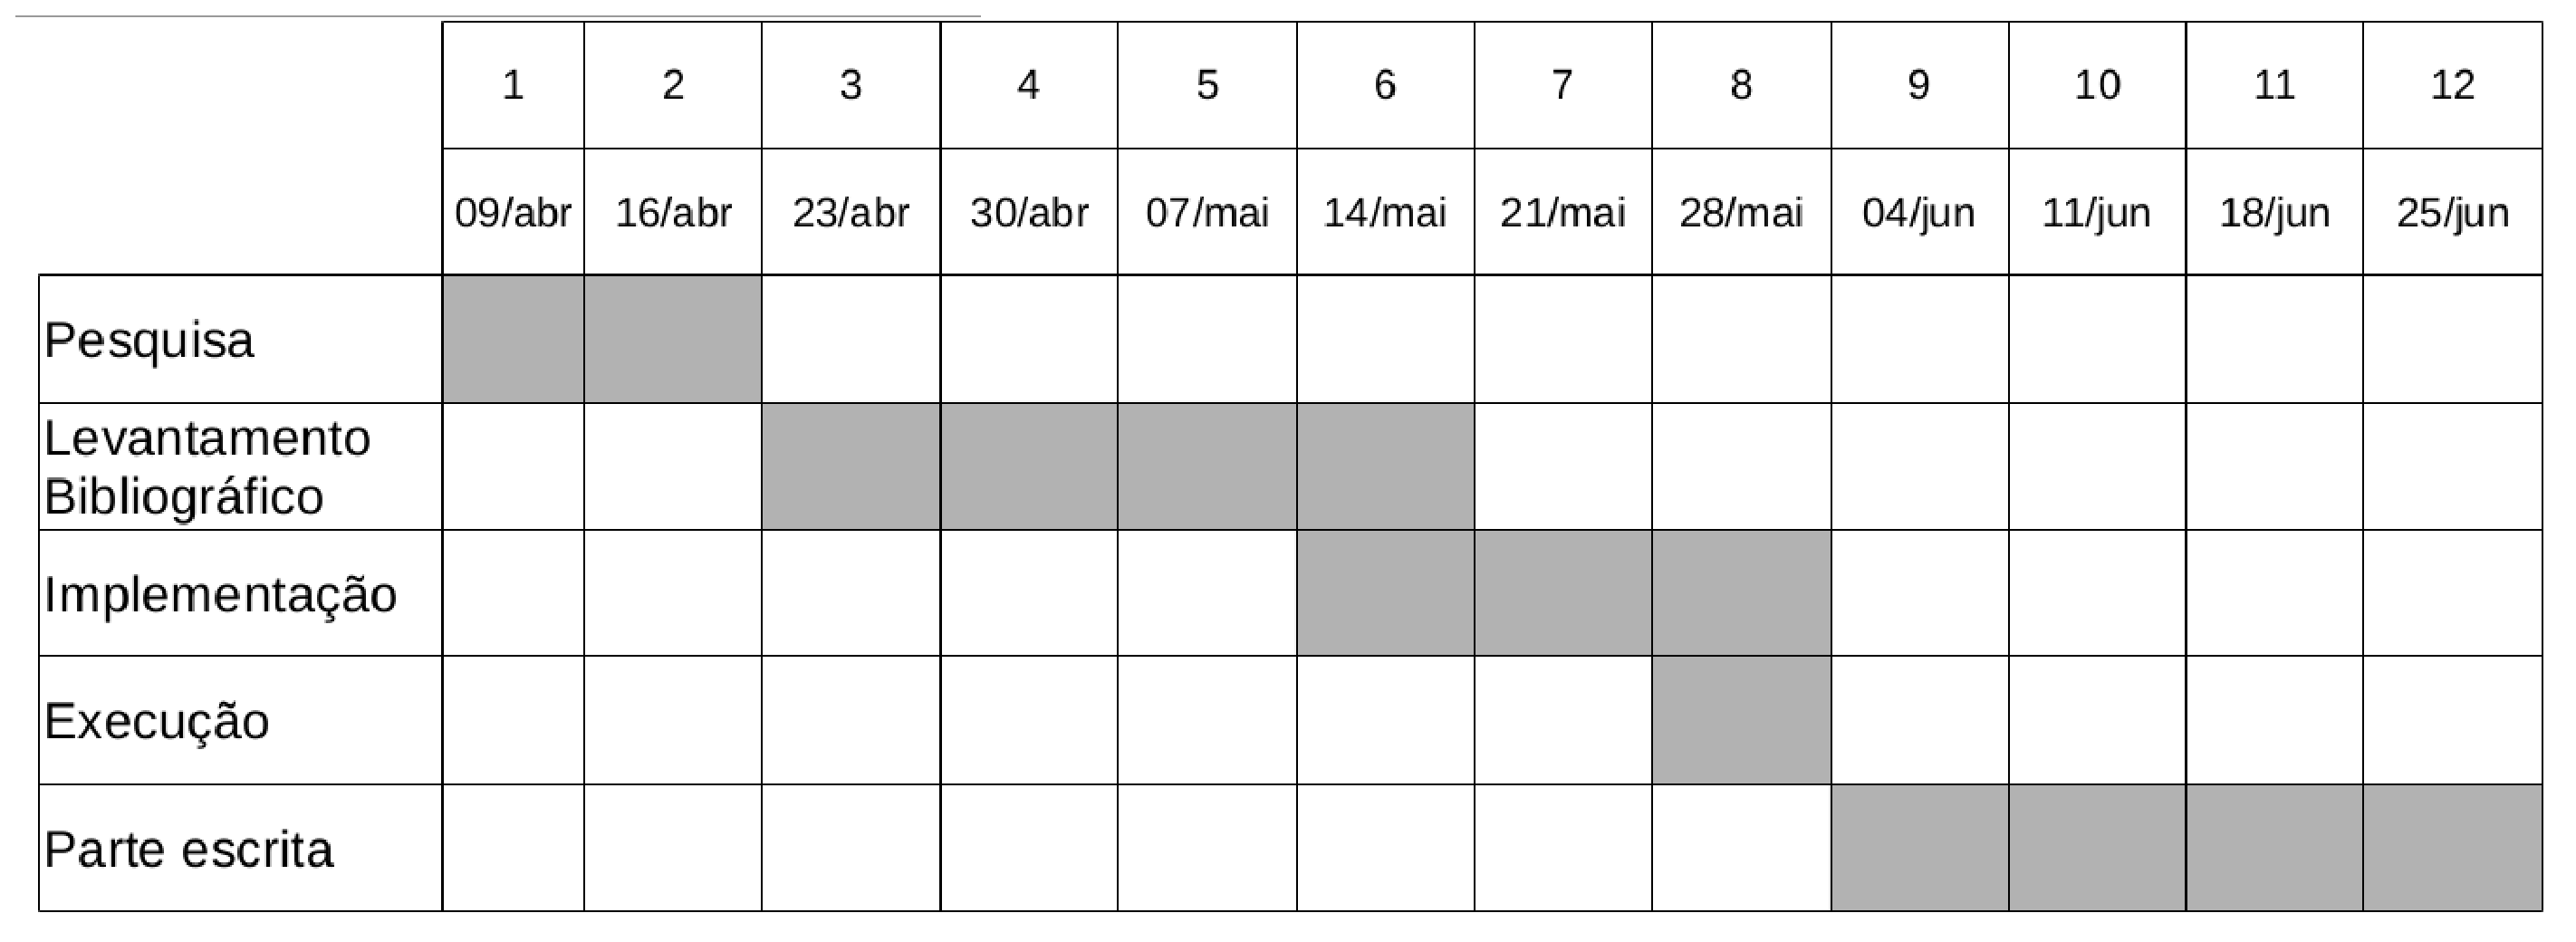
\includegraphics[scale=0.3, bb=0 0 1349 483]{figuras/cronograma.eps}
\end{center}
\caption{Cronograma de trabalho executado.}
\label{fig:cronograma}
\end{figure}
